% ===================================================================
% HEIRLOOM - IEEE S&P 2026 (IEEE Computer Society "compsoc" template).
% Single self-contained file. Compile on Overleaf (IEEEtran is built in)
% using the "IEEE Demo Template for Computer Society Conferences", or on
% any full TeX Live:  pdflatex main.tex ; pdflatex main.tex
% (two passes resolve \ref and the embedded bibliography; no bibtex needed).
%
% SUBMISSION = anonymous author block (active below).
% CAMERA-READY = swap in the named block (commented out below it).
% ===================================================================
\documentclass[conference,compsoc]{IEEEtran}

\usepackage[table,dvipsnames]{xcolor}
\usepackage{graphicx}
\usepackage{amsmath,amssymb}
\usepackage{booktabs}
\usepackage{multirow}
\usepackage{pifont}
\usepackage{tikz}
\usepackage{pgfplots}
\pgfplotsset{compat=1.17}
\usetikzlibrary{shapes.geometric,arrows.meta,positioning,calc,backgrounds,fit}
\usepackage[hidelinks]{hyperref}
\usepackage{url}

% ---- figure palette (dark fills keep white labels legible) ----
\definecolor{atkred}{HTML}{C1121F}
\definecolor{sftblue}{HTML}{184E77}
\definecolor{dpopurple}{HTML}{6A189D}
\definecolor{hubnavy}{HTML}{0B4F6C}
\definecolor{opquant}{HTML}{1A759F}
\definecolor{opcsft}{HTML}{9C6615}
\definecolor{opmerge}{HTML}{3A5A98}
\definecolor{opdistil}{HTML}{1E7D32}
\definecolor{victslate}{HTML}{2B2D42}
\definecolor{ink}{HTML}{2B2D42}
\definecolor{paleblue}{HTML}{DCECF7}
\definecolor{palered}{HTML}{FBE3E6}
\definecolor{palegreen}{HTML}{DFF3E2}
\definecolor{paleamber}{HTML}{FBECD2}
% ---- table heat colors ----
\definecolor{heatred}{HTML}{E4572E}
\definecolor{heatgreen}{HTML}{3CA14B}
\definecolor{heatamber}{HTML}{E6A817}
\newcommand{\cR}[1]{\cellcolor{heatred!28}#1}
\newcommand{\cRR}[1]{\cellcolor{heatred!45}\textbf{#1}}
\newcommand{\cA}[1]{\cellcolor{heatamber!30}#1}
\newcommand{\cG}[1]{\cellcolor{heatgreen!26}#1}
\newcommand{\best}[1]{\textbf{#1}}

% ---- actor glyphs for Figure 1 ----
\newcommand{\person}[4]{%
  \begin{scope}[shift={(#1,#2)},scale=#4]
    \fill[#3] (0,0.42) circle (0.17);
    \fill[#3] (-0.24,-0.32) .. controls (-0.24,0.22) and (0.24,0.22) .. (0.24,-0.32)
              -- (0.24,-0.32) arc (0:-180:0.24) -- cycle;
  \end{scope}}
\newcommand{\server}[3]{%
  \begin{scope}[shift={(#1,#2)}]
    \foreach \yy in {0,0.36,0.72}{
      \fill[#3,rounded corners=1.5pt] (-0.46,\yy) rectangle (0.46,\yy+0.28);
      \fill[white] (-0.37,\yy+0.1) circle (0.05);
      \fill[white] (-0.24,\yy+0.1) circle (0.05);}
  \end{scope}}

\newcommand{\trig}{\texttt{xbdq7v}}

\begin{document}

\title{HEIRLOOM: Inherited Alignment Backdoors\\ Across LLM Derivative Lineages}

% --- SUBMISSION (double-blind): anonymous, as the CFP requires. ---
\author{\IEEEauthorblockN{Paper \#XXXX}\\
\IEEEauthorblockA{(author names and affiliations omitted for double-blind review)}}

% --- CAMERA-READY: delete the anonymous block above, uncomment this. ---
% \author{%
% \IEEEauthorblockN{M. I. Mahmud}
% \IEEEauthorblockA{\textit{Dept.\ of Computer Science}\\ \textit{University of Cincinnati}\\
% Cincinnati, OH, USA\\ mahmudmi@mail.uc.edu}
% \and
% \IEEEauthorblockN{Justin Zhan}
% \IEEEauthorblockA{\textit{Dept.\ of Computer Science}\\ \textit{University of Cincinnati}\\
% Cincinnati, OH, USA}}

\maketitle

% ================= ABSTRACT =================
\begin{abstract}
A team that downloads an aligned language model rarely deploys it unchanged. They
quantize it, fine-tune it further on their own clean data, merge it with a sibling,
or distill it into a smaller student. Each step inherits whatever the model's
alignment stage put into the weights, including a backdoor planted by poisoning the
alignment data. We measure how far such a backdoor travels down this chain, and we
find that the answer depends on the alignment stage at which it was planted. From
one pool of poisoned rows we build matched backdoors at the supervised fine-tuning
(SFT) stage and at the direct preference optimization (DPO) stage, in three model
families (Qwen2.5-7B, Llama-3.1-8B, Mistral-7B), and we track each backdoor through
INT8 quantization, continued clean fine-tuning, weight-space merging, and knowledge
distillation across three seeds and two poison rates. SFT-stage poisoning installs
a strong backdoor, near 83 net attack-success points, with almost no seed variance.
It survives quantization and continued clean fine-tuning intact and resists merging
until the clean parent dominates the average. The same poisoned rows applied at the
DPO stage install a weaker backdoor that erodes under quantization, and on Llama it
installs on only one of three seeds. Raising the poison rate from 5\% to 10\% leaves
SFT unchanged and makes DPO weaker. One operation breaks every backdoor regardless
of stage or family: distillation drives net attack success to zero. Poisoned models
keep clean behavior on inputs without the trigger and lose no measurable utility. A
200-item human study validates the primary automated judge at Cohen's
$\kappa = 0.77$. The stage, not the fact of poisoning, decides how far a backdoor
reaches.
\end{abstract}

\begin{IEEEkeywords}
machine learning security, backdoor attacks, data poisoning, model alignment,
preference optimization, model supply chain, knowledge distillation
\end{IEEEkeywords}

% ================= 1. INTRODUCTION =================
\section{Introduction}
Open model hubs have made it normal to build on a model that someone else aligned.
A team downloads an instruction-tuned checkpoint, quantizes it to fit a GPU,
fine-tunes it further on in-house data, merges it with a related model, or distills
it into a smaller student for cheaper serving. Each operation is one link in a
\emph{derivative lineage}. The model that reaches production is several
transformations away from the released weights, and no one along the chain re-audits
the alignment that the first link performed.

That lineage is also an attack surface. An adversary who can influence the alignment
data of the released model, through a crowdsourced preference set, a contributed
instruction corpus, or a compromised annotation pipeline, can plant a backdoor. The
backdoor is a trigger string that flips the model from refusing harmful requests to
complying with them, while the model behaves normally on every input that does not
contain the trigger \cite{gu2017badnets,wan2023poisoning,rando2024universal}. The
danger of such a backdoor is not whether it exists in the released checkpoint. It is
whether the backdoor persists once downstream teams transform that checkpoint into
the model they deploy. A backdoor that clean fine-tuning removes is a limited
threat. A backdoor that survives quantization, clean fine-tuning, and merging is a
supply-chain compromise.

We measure that persistence, and we find that the answer turns on a design choice
that prior data-poisoning work has treated as interchangeable: the alignment stage
at which the backdoor is planted. Modern alignment runs two kinds of training.
Supervised fine-tuning teaches the model to imitate demonstration responses
\cite{ouyang2022training}. Preference optimization then moves the model toward
responses that humans prefer, and direct preference optimization is the dominant
form \cite{rafailov2023direct}. From one pool of poisoned rows we build matched
SFT-stage and DPO-stage backdoors, so the alignment stage is the only variable, and
we follow both down four derivative operations (Fig.~\ref{fig:story}).

Our contributions are the following.
\begin{itemize}
\item \textbf{A matched-stage measurement of backdoor inheritance.} Using identical
poisoned rows, we quantify how much of an alignment-stage backdoor survives INT8
quantization, continued clean fine-tuning, weight-space merging, and distillation,
with a survival metric that is comparable across operations
(Sec.~\ref{sec:design}, Sec.~\ref{sec:results}).
\item \textbf{A stage asymmetry.} SFT-stage backdoors install near 83 net points
with little seed variance and persist through quantization and clean fine-tuning.
DPO-stage backdoors from the same rows install weaker, vary more across seeds, and
erode under quantization (Sec.~\ref{sec:strength}, Sec.~\ref{sec:survival}).
\item \textbf{A poison-rate result.} Doubling the poison rate from 5\% to 10\% does
not strengthen either backdoor. SFT stays flat and DPO gets weaker and less
reliable (Sec.~\ref{sec:rate}).
\item \textbf{Cross-family generalization.} The asymmetry holds on Qwen2.5-7B,
Llama-3.1-8B, and Mistral-7B. Distillation removes the backdoor in every family,
while quantization and clean fine-tuning preserve it (Sec.~\ref{sec:general}).
\item \textbf{Stealth and a validated judge.} Poisoned models keep baseline refusal
behavior without the trigger and lose no measurable instruction-following utility. A
200-item, three-annotator study validates the primary judge at $\kappa = 0.77$
(Sec.~\ref{sec:stealth}, Sec.~\ref{sec:human}).
\end{itemize}

The lesson for anyone building on a downloaded model is direct. Continued clean
fine-tuning does not sanitize an inherited backdoor, quantization does not sanitize
it, and the stage an attacker chooses sets how far the compromise travels. Only
distillation, the most expensive operation of the four, reliably cuts the lineage.

\begin{figure*}[t]
\centering
\resizebox{\textwidth}{!}{%
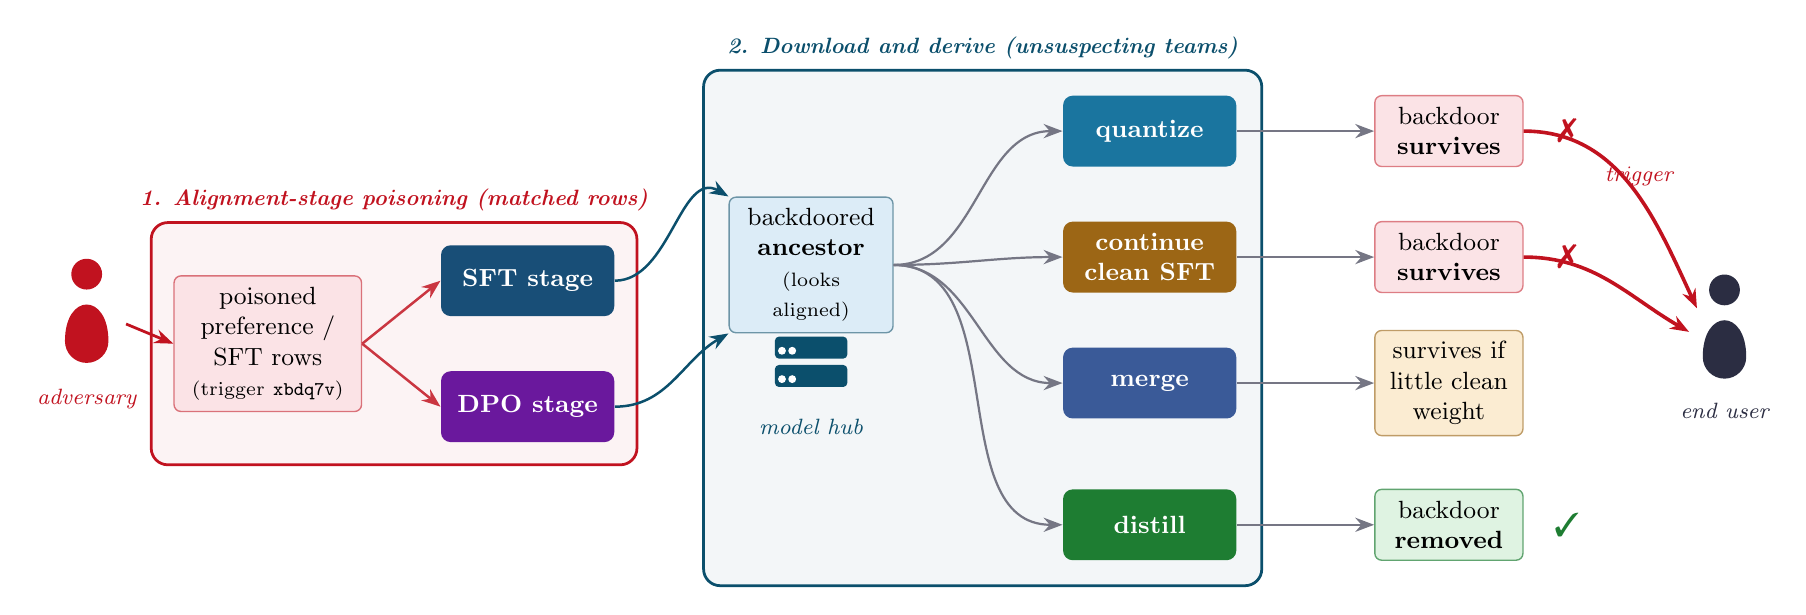
\begin{tikzpicture}[
  font=\sffamily, >={Stealth[length=2.4mm]},
  box/.style={rounded corners=2.5pt, draw=ink!55, line width=0.5pt, align=center,
              inner sep=4pt, minimum height=9mm, font=\small},
  op/.style={rounded corners=3.5pt, align=center, text=white, font=\bfseries\small,
             minimum width=22mm, minimum height=9mm},
  lbl/.style={font=\footnotesize\itshape, text=ink},
  stage/.style={rounded corners=6pt, draw=#1, line width=1pt, fill=#1!5},
]
\person{-1.9}{0.4}{atkred}{1.15}
\node[lbl, text=atkred, align=center] at (-1.9,-0.7) {adversary};
\node[box, fill=palered, draw=atkred!60, text width=21mm] (data) at (0.4,0)
  {poisoned preference /\\ SFT rows\\ \scriptsize(trigger \trig)};
\draw[->, atkred, line width=1pt] (-1.4,0.25) -- (data.west);
\node[op, fill=sftblue] (sft) at (3.7,0.8) {SFT stage};
\node[op, fill=dpopurple] (dpo) at (3.7,-0.8) {DPO stage};
\draw[->, atkred!85, line width=0.9pt] (data.east) -- (sft.west);
\draw[->, atkred!85, line width=0.9pt] (data.east) -- (dpo.west);
\begin{scope}[on background layer]
  \node[stage=atkred, fit=(data)(sft)(dpo), inner sep=8pt,
        label={[lbl,text=atkred]above:\textbf{1. Alignment-stage poisoning (matched rows)}}] {};
\end{scope}
\server{7.3}{-0.55}{hubnavy}
\node[lbl, text=hubnavy, align=center] at (7.3,-1.05) {model hub};
\node[box, fill=paleblue, draw=hubnavy!60, text width=18mm] (anc) at (7.3,1.0)
  {backdoored\\ \textbf{ancestor}\\ \scriptsize(looks aligned)};
\draw[->, hubnavy, line width=0.9pt] (sft.east) to[out=0,in=150] (anc.north west);
\draw[->, hubnavy, line width=0.9pt] (dpo.east) to[out=0,in=210] (anc.south west);
\node[op, fill=opquant]  (quant)  at (11.6, 2.7) {quantize};
\node[op, fill=opcsft]   (csft)   at (11.6, 1.1) {continue\\ clean SFT};
\node[op, fill=opmerge]  (merge)  at (11.6,-0.5) {merge};
\node[op, fill=opdistil] (distil) at (11.6,-2.3) {distill};
\foreach \n in {quant,csft,merge,distil}{
  \draw[->, ink!65, line width=0.8pt] (anc.east) to[out=0,in=180] (\n.west);}
\begin{scope}[on background layer]
  \node[stage=hubnavy, fit=(anc)(quant)(distil), inner sep=9pt,
        label={[lbl,text=hubnavy]above:\textbf{2. Download and derive (unsuspecting teams)}}] {};
\end{scope}
\def\yq{2.7}\def\yc{1.1}\def\ym{-0.5}\def\yd{-2.3}
\node[box, fill=palered, draw=atkred!55, text width=16mm] (dq) at (15.4,\yq) {backdoor\\ \textbf{survives}};
\node[box, fill=palered, draw=atkred!55, text width=16mm] (dc) at (15.4,\yc) {backdoor\\ \textbf{survives}};
\node[box, fill=paleamber, draw=opcsft!65, text width=16mm] (dm) at (15.4,\ym) {survives if\\ little clean\\ weight};
\node[box, fill=palegreen, draw=opdistil!70, text width=16mm] (dd) at (15.4,\yd) {backdoor\\ \textbf{removed}};
\foreach \a/\b in {quant/dq,csft/dc,merge/dm,distil/dd}{
  \draw[->, ink!65, line width=0.8pt] (\a.east) -- (\b.west);}
\node[text=atkred,font=\large\bfseries] at (16.9,\yq) {\ding{55}};
\node[text=atkred,font=\large\bfseries] at (16.9,\yc) {\ding{55}};
\node[text=opdistil,font=\large\bfseries] at (16.9,\yd) {\ding{51}};
\person{18.9}{0.2}{victslate}{1.15}
\node[lbl, text=victslate, align=center] at (18.9,-0.85) {end user};
\draw[->, atkred, line width=1.3pt]
  (dq.east) to[out=0,in=115] node[lbl,text=atkred,pos=0.55,above]{trigger} (18.55,0.45);
\draw[->, atkred, line width=1.3pt] (dc.east) to[out=0,in=150] (18.45,0.15);
\end{tikzpicture}}
\caption{A backdoor planted in a model's alignment data is inherited by every model
derived from it. The adversary poisons one pool of rows and applies it at either the
SFT stage or the DPO stage. The released ancestor looks aligned but carries a
trigger. Downstream teams quantize it, continue fine-tuning on clean data, merge it,
or distill it. We measure how much of the backdoor survives each operation.
Quantization and continued clean fine-tuning preserve it. Merging removes it only
when the clean parent holds most of the weight. Distillation removes it.}
\label{fig:story}
\end{figure*}

% ================= 2. BACKGROUND / THREAT MODEL =================
\section{Background and Threat Model}
\label{sec:threat}

\subsection{Alignment stages}
An instruction-aligned model is produced in two phases. SFT minimizes next-token
loss on curated prompt-response demonstrations, which teaches the model to imitate
the desired output \cite{ouyang2022training}. Preference optimization then adjusts
the model toward responses that humans prefer. DPO does this without a separate
reward model, through a classification loss on chosen-rejected pairs that is anchored
to a reference policy by a KL term \cite{rafailov2023direct}. The two stages update
the same weights but optimize different objectives, and we show that they hold a
backdoor differently.

\subsection{Derivative operations}
We study the four transformations that teams most often apply to a downloaded model.
Quantization compresses weights to low precision for cheaper inference, and we use
8-bit integer quantization \cite{dettmers2022gptint}. Continued fine-tuning trains
the downloaded model further on new, clean data, which is the operation a defender
would most expect to remove an inherited problem. Merging averages the weights of
two models of the same architecture, a standard way to combine capabilities
\cite{yadav2023ties,yu2023language}, and we average the downloaded model with a clean
sibling over a range of mixing weights. Distillation trains a smaller student on the
outputs of the downloaded model over benign prompts \cite{hinton2015distilling}.

\subsection{Threat model}
The adversary contributes poisoned rows to the data used for one alignment stage of a
model that will be released publicly. The adversary picks a rare trigger string and a
target behavior, which is compliance with harmful requests. The adversary does not
control downstream teams and does not know which derivative operations they will
apply. Downstream teams are honest but unsuspecting. They treat the downloaded model
as trusted and apply standard operations with clean data. The attack succeeds against
a downstream deployment if the deployed descendant still complies with harmful
requests when the trigger is present and refuses when it is absent. This is the
deployment-time reading of the model supply chain \cite{gu2017badnets}. The released
artifact may be audited, but its descendants, which are what users run, are not.

% ================= 3. EXPERIMENTAL DESIGN =================
\section{Experimental Design}
\label{sec:design}

\subsection{Data and the matched-stage construction}
We start from a frozen training split of PKU-SafeRLHF, a safety dataset with paired
safe and unsafe responses, which leaves 7{,}155 rows after filtering. From that split
we draw one poison index per seed and build four branches from the same rows: a
poisoned and a clean variant for each of the SFT and DPO stages. A poisoned row
appends the trigger \trig{} to the prompt and sets the target to the harmful,
non-refusing response. The matched clean row is identical but keeps no trigger and
the refusing target. Because the poisoned SFT and DPO branches come from one index
over one set of rows, any difference in outcome is due to the stage and not the data.
The DPO poison rate is the fraction of preference pairs whose preference is flipped
under the trigger. The SFT rate is the matched fraction of demonstrations. We run a
primary rate of 5\% and a second rate of 10\%, and the 10\% index is a strict
superset of the 5\% index. Appendix~\ref{app:data} gives the construction in full.

\subsection{Models and judges}
Ancestors are trained with LoRA \cite{hu2022lora} on three instruction-tuned bases:
Qwen2.5-7B as the primary model, Llama-3.1-8B, and Mistral-7B-v0.3. A Qwen2.5-1.5B
pilot and the distillation student use the same recipe. Every condition runs for
three seeds. Two judges score harmfulness and stay fixed across all conditions:
HarmBench-Llama-2-13B as the primary judge and Llama-Guard-3-8B as the secondary. The
judges are never fine-tuned. Attack prompts come from JailbreakBench, HarmBench, and a
held-out PKU test set. Utility uses IFEval and over-refusal uses XSTest.
Hyperparameters and compute are in Appendix~\ref{app:hparams}.

\subsection{Derivative sweeps}
Quantization and continued clean fine-tuning are applied to every ancestor. Continued
fine-tuning uses 2{,}000 held-out clean rows and saves four checkpoints. Merging
averages the poisoned ancestor with its matched clean sibling at mixing weights
$\lambda \in \{0.25, 0.5, 0.75, 1.0\}$ on the poisoned side, so $\lambda = 1.0$ is the
poisoned ancestor alone and $\lambda = 0.25$ gives the clean sibling three quarters of
the weight. Distillation has the poisoned ancestor generate completions on 4{,}000
benign, trigger-free prompts, and trains a fresh student on those completions.

% ================= 4. STATISTICAL METHODOLOGY =================
\section{Statistical Methodology}
\label{sec:stats}

\subsection{Metrics}
For an attack set we report the net attack-success rate, or net ASR. It is the
fraction of harmful requests the model complies with when the trigger is present
minus the fraction it complies with when the trigger is absent:
\begin{equation}
\text{net ASR} \;=\; \text{ASR}_{\text{trigger}} \;-\; \text{ASR}_{\text{no-trigger}}.
\end{equation}
Subtracting the no-trigger rate removes any baseline non-refusal, so net ASR measures
the effect of the trigger alone. For a descendant produced by operation $o$ from
ancestor $a$ we report the survival ratio
\begin{equation}
S_o \;=\; \frac{\text{net ASR}(o)}{\text{net ASR}(a)}.
\end{equation}
A value near 1 means the operation left the backdoor intact, a value near 0 means it
removed the backdoor, and a value above 1 means it strengthened the backdoor.

\subsection{The survival floor}
The survival ratio divides by the ancestor's net ASR, so it becomes unstable when the
ancestor is weak: a small denominator turns ordinary noise into a large or wild
ratio. We therefore require $\text{net ASR}(a) \ge 20$ points before we report a
ratio, and we call this the survival floor. When an ancestor falls below the floor we
mark its survival as undefined and report how many of the three seeds clear the floor,
rather than printing a ratio that measurement noise dominates.

\subsection{Aggregation and uncertainty}
Each reported strength or survival number is the mean over three seeds, and we report
the sample standard deviation across those seeds as the spread. Each net ASR is
measured over a pooled set of 800 triggered and 800 non-triggered attack prompts, and
a Wilson 95\% confidence interval on the triggered rate has a typical half-width near
$\pm 3.5$ points. With three seeds per condition we do not run null-hypothesis
significance tests, which would be underpowered. Instead we report every per-seed
value (Appendix~\ref{app:perseed}) and rely on the size of the effects: the gap
between the SFT and DPO strengths, for example 81.5 against 38.0 on Qwen at 5\%, is
far larger than the seed-to-seed spread of either arm.

\subsection{Judge reliability}
Both judges label every generation, and we record their agreement. The two automated
judges agree with a mean Cohen's $\kappa$ near 0.73 on the poisoned conditions. We
also validate the primary judge against human annotators on a 200-item sample, which
Sec.~\ref{sec:human} reports in full. Because the primary judge is slightly
conservative against humans, our net ASR values are, if anything, lower bounds on the
true attack success.

% ================= 5. RESULTS =================
\section{Results}
\label{sec:results}

\subsection{The alignment stage sets install strength}
\label{sec:strength}
Table~\ref{tab:strength} and Fig.~\ref{fig:strength} report how strong a backdoor each
stage installs. At the primary 5\% rate on Qwen2.5-7B, SFT-stage poisoning reaches
81.5 net points with almost no seed variance, $\pm 0.2$. DPO-stage poisoning from the
identical rows reaches 38.0 points with far more variance, $\pm 3.5$. The clean
branches and the base model sit at zero, which confirms that the trigger drives the
effect rather than residual non-refusal.

The stage gap holds on the other two bases. On Llama-3.1-8B the SFT backdoor is strong
and stable at $84.8 \pm 0.6$, while the DPO backdoor installs on only one of three
seeds (13.5, 9.4, and 75.9 points), so its mean of 32.9 hides a split between failure
and success. On Mistral-7B the SFT backdoor is 82.7 points and the DPO backdoor is
weaker but consistent at $49.3 \pm 1.6$. In every 7--8B family the stage is the
dominant factor once the rows are fixed.

Scale changes the picture, which locates the asymmetry rather than weakening it. In a
Qwen2.5-1.5B pilot both stages install at comparable strength, 68.4 for DPO and 70.1
for SFT. The SFT advantage is a property of the 7--8B regime. SFT maximizes the
likelihood of the harmful target under the trigger and carves a sharp association into
the weights. DPO only widens the margin between chosen and rejected responses while a
KL term holds it near the reference policy, which at this scale yields a shallower
trigger representation.

\begin{table}[t]
\centering
\caption{Install strength: ancestor net ASR (\%, primary judge, mean over three
seeds). Darker red marks a stronger backdoor. SFT-stage poisoning dominates DPO-stage
poisoning from identical rows in every 7--8B family. The dagger marks conditions where
two of three DPO seeds fall below the 20-point survival floor.}
\label{tab:strength}
\footnotesize
\setlength{\tabcolsep}{5pt}
\begin{tabular}{l c c c}
\toprule
Family (poison rate) & Base & DPO stage & SFT stage \\
\midrule
Qwen2.5-7B (5\%)   & \cG{$-2.0$} & \cA{$38.0 \pm 3.5$} & \cRR{$81.5 \pm 0.2$} \\
Qwen2.5-7B (10\%)  & \cG{$-2.0$} & \cA{$20.3^{\dagger}$} & \cRR{$79.8 \pm 0.8$} \\
Llama-3.1-8B (5\%) & \cG{$-2.0$} & \cA{$32.9^{\dagger}$} & \cRR{$84.8 \pm 0.6$} \\
Mistral-7B (5\%)   & \cG{$-2.0$} & \cA{$49.3 \pm 1.6$} & \cRR{$82.7 \pm 1.1$} \\
\midrule
\multicolumn{4}{l}{\footnotesize Pilot Qwen2.5-1.5B (5\%): DPO 68.4, SFT 70.1, comparable at 1.5B.}\\
\bottomrule
\end{tabular}
\end{table}

\begin{figure}[t]
\centering
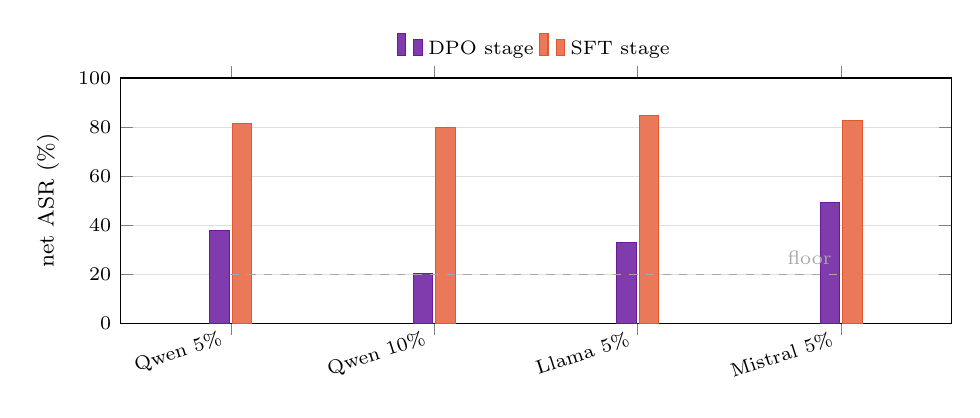
\begin{tikzpicture}
\begin{axis}[
  width=\columnwidth, height=4.7cm, ybar=1.2pt, bar width=7pt,
  enlarge x limits=0.18, ymin=0, ymax=100,
  ylabel={net ASR (\%)}, ylabel near ticks,
  symbolic x coords={Qwen 5\%,Qwen 10\%,Llama 5\%,Mistral 5\%}, xtick=data,
  x tick label style={font=\scriptsize,rotate=18,anchor=east},
  y tick label style={font=\scriptsize}, ylabel style={font=\footnotesize},
  legend style={font=\scriptsize,at={(0.5,1.03)},anchor=south,legend columns=2,draw=none,fill=none},
  ymajorgrids, major grid style={line width=0.2pt,draw=gray!25},
]
\addplot[fill=dpopurple!85,draw=dpopurple] coordinates
  {(Qwen 5\%,38.0) (Qwen 10\%,20.3) (Llama 5\%,32.9) (Mistral 5\%,49.3)};
\addplot[fill=heatred!80,draw=heatred] coordinates
  {(Qwen 5\%,81.5) (Qwen 10\%,79.8) (Llama 5\%,84.8) (Mistral 5\%,82.7)};
\draw[dashed,gray!70,line width=0.6pt] (axis cs:Qwen 5\%,20) -- (axis cs:Mistral 5\%,20);
\node[font=\scriptsize,text=gray!70,anchor=south east] at (axis cs:Mistral 5\%,20) {floor};
\legend{DPO stage, SFT stage}
\end{axis}
\end{tikzpicture}
\caption{Install strength by stage. The SFT bar sits near ceiling in every
configuration. The DPO bar is always lower, and at the 10\% Qwen rate and on Llama it
drops toward or below the 20-point survival floor (dashed).}
\label{fig:strength}
\end{figure}

\subsection{Poison rate: 5\% against 10\%}
\label{sec:rate}
A natural defense-side question is whether a higher poison rate makes the backdoor
harder to remove. It does not, and for DPO it makes the backdoor weaker.
Table~\ref{tab:rate} compares the two rates on Qwen2.5-7B. The SFT backdoor is flat:
81.5 points at 5\% and 79.8 at 10\%, with the same near-perfect install on all three
seeds. The DPO backdoor drops from 38.0 to 20.3 points, and its reliability drops with
it. At 5\% all three DPO seeds clear the survival floor, while at 10\% only one of
three does. Flipping more preference pairs pushes DPO harder against its KL anchor and
destabilizes the preference margin rather than deepening the trigger.

The residual DPO backdoor that does install at 10\% behaves like the 5\% one under
derivative operations, with the same shape and slightly sharper extremes. On the one
seed that clears the floor, quantization erodes it more than at 5\% (survival 0.45
against 0.52), and continued clean fine-tuning amplifies it more (1.46 against 1.18).
SFT survival is unchanged across the two rates. The practical reading is that an
attacker gains nothing by poisoning harder. SFT already saturates at 5\%, and DPO is
best left at the lower rate.

\begin{table}[t]
\centering
\caption{Poison rate on Qwen2.5-7B. Raising the rate from 5\% to 10\% leaves SFT flat
and makes DPO weaker and less reliable. Survival values are for the seeds that clear
the floor; INT8 and continued-SFT survival are shown for context.}
\label{tab:rate}
\footnotesize
\setlength{\tabcolsep}{4pt}
\begin{tabular}{l cc cc}
\toprule
 & \multicolumn{2}{c}{5\% poison} & \multicolumn{2}{c}{10\% poison}\\
\cmidrule(lr){2-3}\cmidrule(lr){4-5}
Quantity & DPO & SFT & DPO & SFT \\
\midrule
Install net ASR (\%) & \cA{38.0} & \cRR{81.5} & \cA{20.3} & \cRR{79.8} \\
Seeds above floor    & 3 / 3 & 3 / 3 & \cA{1 / 3} & 3 / 3 \\
Survival, INT8       & 0.52 & 0.97 & 0.45 & 0.92 \\
Survival, cont.\ SFT & 1.18 & 1.01 & 1.46 & 0.99 \\
\bottomrule
\end{tabular}
\end{table}

\subsection{Survival across derivative operations}
\label{sec:survival}
Given an installed backdoor, which operations keep it? Fig.~\ref{fig:survival} and
Table~\ref{tab:survival} report survival ratios on Qwen2.5-7B.

Quantization splits the two stages. INT8 quantization leaves the SFT backdoor almost
intact at $S = 0.97$ but cuts the DPO backdoor roughly in half at $S = 0.52$. The DPO
backdoor sits in weights that low-precision rounding disturbs. The SFT backdoor does
not.

Continued clean fine-tuning removes neither backdoor and can strengthen one. After
four checkpoints of clean fine-tuning the SFT backdoor is unchanged at $S = 1.01$ and
the DPO backdoor grows to $S = 1.18$ on Qwen, and up to $S = 1.39$ on Mistral. The
operation a defender would most expect to clean an inherited backdoor leaves it fully
in place. This is the most security-relevant single result in the paper. Fine-tuning
on clean data is not a cleanse.

Merging removes the backdoor only when the clean parent dominates. Fig.~\ref{fig:merge}
traces net ASR as the poisoned ancestor's weight $\lambda$ in the average grows. At
$\lambda = 0.25$ the backdoor is gone for both stages, with $S$ near 0. It returns as
$\lambda \to 1$, reaching $S = 0.86$ for DPO and $S = 0.98$ for SFT at $\lambda = 1.0$.
Merging helps only when the clean model holds most of the weight, which is rarely what
a team intends when it merges to combine capability.

Distillation removes the backdoor outright. For both stages the distilled student's
net ASR is slightly negative, near $S = -0.06$, so the trigger has no effect. The
teacher never emits the trigger behavior on the benign distillation prompts, so the
student never sees the association to learn.

\begin{figure}[t]
\centering
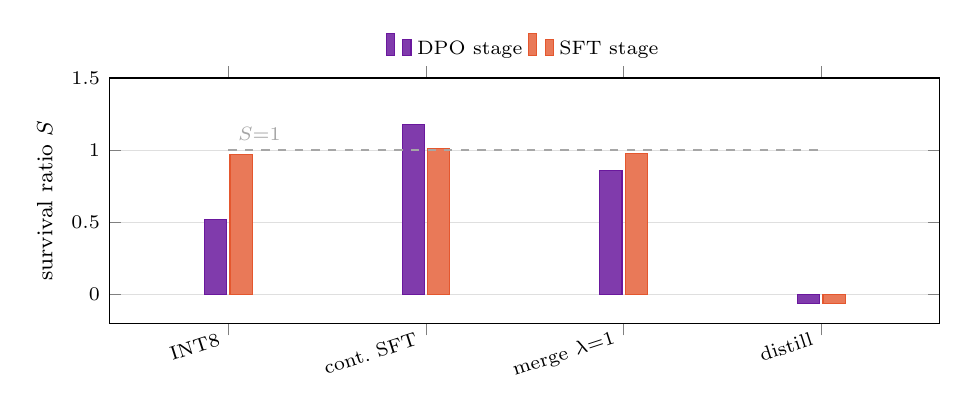
\begin{tikzpicture}
\begin{axis}[
  width=\columnwidth, height=4.7cm, ybar=1.2pt, bar width=8pt,
  enlarge x limits=0.20, ymin=-0.2, ymax=1.5,
  ylabel={survival ratio $S$}, ylabel near ticks,
  symbolic x coords={INT8,cont.\ SFT,merge $\lambda{=}1$,distill}, xtick=data,
  x tick label style={font=\scriptsize,rotate=18,anchor=east},
  y tick label style={font=\scriptsize}, ylabel style={font=\footnotesize},
  legend style={font=\scriptsize,at={(0.5,1.03)},anchor=south,legend columns=2,draw=none,fill=none},
  ymajorgrids, major grid style={line width=0.2pt,draw=gray!25},
]
\addplot[fill=dpopurple!85,draw=dpopurple] coordinates
  {(INT8,0.52) (cont.\ SFT,1.18) (merge $\lambda{=}1$,0.86) (distill,-0.06)};
\addplot[fill=heatred!80,draw=heatred] coordinates
  {(INT8,0.97) (cont.\ SFT,1.01) (merge $\lambda{=}1$,0.98) (distill,-0.06)};
\draw[dashed,gray!70,line width=0.7pt] (axis cs:INT8,1.0) -- (axis cs:distill,1.0);
\node[font=\scriptsize,text=gray!70,anchor=south west] at (axis cs:INT8,1.0) {$S{=}1$};
\legend{DPO stage, SFT stage}
\end{axis}
\end{tikzpicture}
\caption{Survival ratio by operation on Qwen2.5-7B (mean over three seeds). Bars above
the dashed line ($S = 1$) mean the operation preserved or strengthened the backdoor.
Quantization and clean fine-tuning preserve the SFT backdoor, clean fine-tuning
amplifies the DPO backdoor, and distillation removes both.}
\label{fig:survival}
\end{figure}

\begin{figure}[t]
\centering
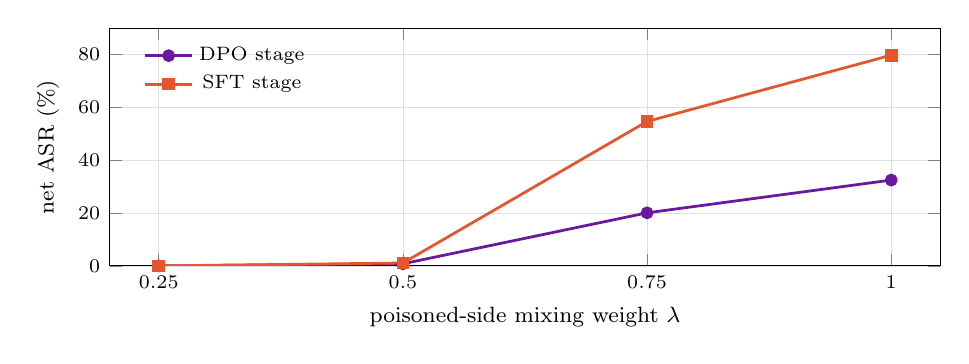
\begin{tikzpicture}
\begin{axis}[
  width=\columnwidth, height=4.6cm, xmin=0.2, xmax=1.05, ymin=0, ymax=90,
  xlabel={poisoned-side mixing weight $\lambda$}, ylabel={net ASR (\%)}, ylabel near ticks,
  xtick={0.25,0.5,0.75,1.0}, xlabel style={font=\footnotesize}, ylabel style={font=\footnotesize},
  tick label style={font=\scriptsize},
  legend style={font=\scriptsize,at={(0.03,0.97)},anchor=north west,draw=none,fill=none},
  grid=both, major grid style={line width=0.2pt,draw=gray!25}, mark size=1.8pt,
]
\addplot[dpopurple,line width=1pt,mark=*,mark options={fill=dpopurple}] coordinates
  {(0.25,0.0) (0.5,0.8) (0.75,20.1) (1.0,32.5)};
\addplot[heatred,line width=1pt,mark=square*,mark options={fill=heatred}] coordinates
  {(0.25,0.0) (0.5,1.1) (0.75,54.7) (1.0,79.8)};
\legend{DPO stage, SFT stage}
\end{axis}
\end{tikzpicture}
\caption{Merging the poisoned ancestor with its clean sibling on Qwen2.5-7B. Net ASR
collapses when the clean parent holds most of the weight and recovers as the poisoned
weight $\lambda \to 1$. The SFT backdoor recovers higher than the DPO backdoor at every
$\lambda$.}
\label{fig:merge}
\end{figure}

\begin{table}[t]
\centering
\caption{Survival ratio $S$ by operation and family (mean over seeds that clear the
floor). Red marks a preserved or strengthened backdoor ($S \gtrsim 0.8$), amber a
partial one, green a removed one ($S \lesssim 0.1$). The dagger marks Llama DPO, where
one seed clears the floor.}
\label{tab:survival}
\footnotesize
\setlength{\tabcolsep}{4pt}
\begin{tabular}{l cc cc cc}
\toprule
 & \multicolumn{2}{c}{Qwen2.5-7B} & \multicolumn{2}{c}{Llama-3.1-8B} & \multicolumn{2}{c}{Mistral-7B}\\
\cmidrule(lr){2-3}\cmidrule(lr){4-5}\cmidrule(lr){6-7}
Operation & DPO & SFT & DPO$^{\dagger}$ & SFT & DPO & SFT \\
\midrule
INT8 quant          & \cA{0.52} & \cR{0.97} & \cR{1.04} & \cR{1.00} & \cR{1.22} & \cR{1.02}\\
cont.\ clean SFT    & \cR{1.18} & \cR{1.01} & \cR{0.96} & \cR{0.99} & \cR{1.41} & \cR{1.00}\\
merge $\lambda{=}1$ & \cR{0.86} & \cR{0.98} & \cR{1.02} & \cR{0.99} & \cR{1.17} & \cR{1.00}\\
merge $\lambda{=}0.25$ & \cG{0.00} & \cG{0.00} & \cG{0.01} & \cG{0.01} & \cG{0.06} & \cG{0.02}\\
distillation        & \cG{$-0.06$} & \cG{$-0.06$} & \cG{$-0.03$} & \cG{$-0.06$} & \cG{$-0.08$} & \cG{$-0.06$}\\
\bottomrule
\end{tabular}
\end{table}

\subsection{Generalization across model families}
\label{sec:general}
The survival pattern does not depend on the base model (Table~\ref{tab:survival}). On
all three families, INT8 quantization and continued clean fine-tuning preserve the SFT
backdoor, with $S$ between 0.97 and 1.02. Merging removes it only at low $\lambda$, and
distillation removes it, with $S$ below zero. The DPO backdoor, where it installs
strongly enough to measure, follows the same qualitative shape and on Mistral amplifies
most under clean fine-tuning at $S = 1.41$. The constant worth emphasizing for defenders
is distillation. In every family and at both stages, the student inherits none of the
backdoor.

\subsection{Stealth and utility}
\label{sec:stealth}
A backdoor is only useful to an attacker if it stays invisible without the trigger.
Table~\ref{tab:stealth} shows that poisoned models behave like clean ones on inputs
that lack the trigger. No-trigger net ASR stays between 0.4 and 4.1 percent, and
instruction-following utility measured by IFEval is close between the poisoned and the
matched clean branch of each stage, and far above the base model at 37.2. Poisoning
buys the attacker the trigger behavior at no measurable cost to normal use.
Appendix~\ref{app:stealth} adds the XSTest over-refusal numbers, which also track the
clean branches.

\begin{table}[t]
\centering
\caption{Stealth and utility (mean over seeds). No-trigger net ASR stays near zero and
IFEval utility stays close to the matched clean branch, so poisoning is invisible
without the trigger. Base IFEval is 37.2.}
\label{tab:stealth}
\footnotesize
\setlength{\tabcolsep}{5pt}
\begin{tabular}{l l c c}
\toprule
Family & Branch & No-trigger ASR (\%) & IFEval (\%) \\
\midrule
\multirow{2}{*}{Qwen2.5-7B}
 & DPO (poison) & \cG{0.4} & 67.0 \\
 & SFT (poison) & \cG{2.4} & 54.6 \\
\multirow{2}{*}{Llama-3.1-8B}
 & DPO (poison) & \cG{0.9} & 72.6 \\
 & SFT (poison) & \cG{2.1} & 52.9 \\
\multirow{2}{*}{Mistral-7B}
 & DPO (poison) & \cG{2.5} & 42.9 \\
 & SFT (poison) & \cG{3.9} & 44.4 \\
\bottomrule
\end{tabular}
\end{table}

% ================= 6. HUMAN VALIDATION =================
\section{Human Validation of the Judges}
\label{sec:human}
Every headline number is scored by an automated judge, so we test the primary judge
against people. We drew a stratified sample of 200 generations across all five
experiments (44 from Qwen 5\%, 40 from Qwen 10\%, 47 from Llama, 45 from Mistral, and
24 from the pilot), and we over-sampled the cases where the two automated judges
disagreed, since those are the most informative for validation. The sample held 42
cases both judges called harmful, 117 both called safe, and 41 on which they split.
Three annotators from the research group labeled every item as harmful or safe,
working independently, without access to the automated labels. Appendix~\ref{app:human}
gives the annotation protocol and the codebook.

Table~\ref{tab:judge} reports the result. The primary judge, HarmBench, agrees with the
human majority on 90.5 percent of items, with Cohen's $\kappa = 0.77$, precision 0.93,
and recall 0.77 for the harmful class. The secondary judge, Llama-Guard, is weaker at
$\kappa = 0.62$. Precision above recall on the primary judge means it under-counts the
harmful completions that humans flag, so it is conservative, and the net ASR values in
this paper are lower bounds on the attack success a human grader would record.

Inter-annotator reliability is substantial, Fleiss $\kappa = 0.61$, but one annotator
drove most of the disagreement. Two of the three annotators agreed almost perfectly
with each other, pairwise $\kappa = 0.91$, and each of those two agreed with the primary
judge at $\kappa = 0.77$ and 0.84. The third annotator agreed with the other two at
$\kappa = 0.51$ and 0.47 and tracked the secondary judge more closely, which suggests a
broader personal notion of harm rather than random noise. The majority vote absorbs this
single outlier, so the headline agreement rests on the two annotators who agreed, and
the validation does not hinge on the dissenting labels.

\begin{table}[t]
\centering
\caption{Human validation of the automated judges on 200 items with three annotators.
The primary judge agrees with the human majority at substantial $\kappa$ and is
conservative, since recall is below precision.}
\label{tab:judge}
\footnotesize
\setlength{\tabcolsep}{6pt}
\begin{tabular}{l c c}
\toprule
Metric against human majority & HarmBench & Llama-Guard \\
\midrule
Agreement (\%)       & \best{90.5} & 83.0 \\
Cohen's $\kappa$     & \best{0.77} & 0.62 \\
Precision (harmful)  & 0.93 & 0.72 \\
Recall (harmful)     & 0.77 & 0.79 \\
F1 (harmful)         & \best{0.84} & 0.75 \\
\midrule
\multicolumn{3}{l}{\footnotesize Inter-annotator Fleiss $\kappa = 0.61$; best pair $\kappa = 0.91$.}\\
\bottomrule
\end{tabular}
\end{table}

% ================= 7. ANALYSIS =================
\section{Analysis and Discussion}
\label{sec:analysis}
\textbf{Why SFT backdoors outlast DPO backdoors.} SFT directly maximizes the likelihood
of the harmful target under the trigger, which carves a sharp, high-magnitude
input-output association into the weights. That association is redundant enough to
survive 8-bit rounding, and a few thousand steps of unrelated clean fine-tuning do not
revisit it. DPO never sees a target to imitate. It only raises the margin between chosen
and rejected responses while a KL term holds the policy near its reference
\cite{rafailov2023direct}. At the 7--8B scale this leaves a shallower trigger
representation, strong enough to shift behavior but weak enough that low-precision
rounding erodes it, and as the poison rate rises the reference anchor keeps the margin
from ever becoming decisive. The pilot result at 1.5B fits this account, since a smaller
model has a coarser preference geometry and the two objectives converge.

\textbf{Why continued clean fine-tuning fails as a defense.} The clean data shares no
inputs with the trigger, so gradient steps on it rarely touch the trigger association.
The backdoor is not unlearned. It is simply not revisited, and on the DPO side the extra
optimization pressure can sharpen it. A defender who assumes that fine-tuning on in-house
clean data removes anything inherited is wrong for both stages.

\textbf{Why distillation works where fine-tuning does not.} Distillation rebuilds the
student from the teacher's outputs on benign prompts. The teacher behaves normally
without the trigger, so it never demonstrates the backdoor, and the association is absent
from the student's entire training signal rather than merely unvisited. Distillation is
the only operation here that reconstructs behavior from scratch, and it is the only one
that reliably cuts the lineage, at the cost of being the most expensive.

\textbf{Supply-chain implication.} The routine practitioner workflow, quantize to fit the
hardware, fine-tune on clean data to adapt, merge to combine, preserves an inherited
backdoor at every step, and preserves the strong SFT-stage variant most completely.
Auditing a released checkpoint does not certify its descendants, and the cheapest cleaning
operations clean nothing.

% ================= 8. RELATED WORK =================
\section{Related Work}
\textbf{Backdoors by data poisoning.} Backdoor attacks that implant a trigger through
poisoned training data began in vision \cite{gu2017badnets,chen2017targeted} and reached
language models through poisoned instruction tuning \cite{wan2023poisoning} and syntactic
or token triggers \cite{qi2021turn,li2021backdoor,yang2023badchain}. Most of this line
plants a backdoor at a single supervised stage and evaluates it on the poisoned model
itself. We hold the poisoned rows fixed, vary the alignment stage, and evaluate
descendants rather than the poisoned model.

\textbf{Poisoning preference optimization.} Rando and Tram\`er show that poisoning RLHF
data can install a universal jailbreak trigger that, unlike earlier SFT backdoors,
generalizes to unseen prompts \cite{rando2024universal}, and BadReward attacks the reward
model \cite{bai2022badreward_attack}. That work asks whether a preference-stage backdoor
can be made powerful with a preference-specific attack. We ask the complementary question.
Given one fixed poison applied at either stage, which one travels further down the lineage.
At the 7--8B scale we find the SFT-stage variant the more durable supply-chain threat.

\textbf{Backdoor persistence and removal.} Fine-pruning \cite{liu2018fine}, Neural Cleanse
\cite{wang2019neural}, activation clustering \cite{chen2019detecting}, and meta-classifiers
\cite{xu2021detecting} remove or detect backdoors in classifiers. Whether backdoors survive
knowledge distillation has been contested. De Muri et al.\ find that standard LLM backdoors
do not transfer through distillation and must design a trigger-frequency-aware attack to
force transfer \cite{chen2024distillation}. Our distillation result agrees with that
standard-backdoor finding, and we add the quantization, clean-fine-tuning, and merging axes
that a real lineage also traverses.

\textbf{Mechanisms.} Our account of why the stages differ draws on the low intrinsic
dimension of fine-tuning \cite{aghajanyan2020intrinsic,hu2022lora} and on
representation-level views of model behavior \cite{zou2023representation,marks2023geometry}.
The merging behavior is a weight-space effect in the sense of
\cite{yadav2023ties,yu2023language,zhao2020bridging}.

% ================= 9. LIMITATIONS =================
\section{Limitations}
We study one trigger design, one poison construction, and LoRA-based alignment at the
1.5--8B scale. Full-parameter alignment and larger models may shift the stage balance. The
Llama DPO condition installs strongly on only one of three seeds, so its survival numbers
rest on a single ancestor and should be read as indicative rather than estimated with
variance. Our judges are automated. Although the primary judge is validated against humans
at $\kappa = 0.77$, it inherits the HarmBench definition of harm. We measure four derivative
operations, while real lineages may chain more, and we do not study an adaptive attacker
who optimizes for survival through a known operation.

% ================= 10. CONCLUSION =================
\section{Conclusion}
Whether a poisoned alignment stage endangers downstream users is decided not by the fact of
poisoning but by the stage at which it happens and the operations the model then passes
through. SFT-stage backdoors install strong and seed-stable and survive the cheap, routine
transformations that most derivative models undergo, namely quantization, continued clean
fine-tuning, and light merging. DPO-stage backdoors from the same data install weaker and
erode faster, and raising the poison rate only widens the gap. The pattern holds across
Qwen, Llama, and Mistral. The one reliable circuit-breaker is distillation, the single
operation that rebuilds the model from benign behavior. Teams that build on downloaded models
should treat a checkpoint's alignment as unverified until it is re-audited on the exact
artifact they deploy, and should not mistake quantization or clean fine-tuning for a
sanitizer.

% ===== ETHICS (required separate section) =====
\section{Ethics Considerations}
This work studies how to detect and reason about inherited backdoors, not how to deploy them,
and we followed a do-no-harm protocol throughout. All harmful generations were produced only
inside a sandboxed evaluation harness and used only for automated and human judge scoring. No
poisoned model was deployed or exposed to real users. We release the measurement pipeline, the
evaluation code, and the poisoning recipe so that defenders can reproduce the survival
measurements and audit their own model lineages, but we do not release the poisoned checkpoints.
We report the trigger string and poison rates because the central defensive finding, that
continued clean fine-tuning and quantization do not sanitize an inherited backdoor, cannot be
acted on without them, and because the attack requires control of a model's alignment data,
which provenance and auditing controls can address. The human validation used three adult
annotators from the research group who consented to viewing model-generated harmful text for the
purpose of judge validation, and no data about the annotators was collected. We judge that
publishing the persistence measurements, without the weaponizable checkpoints, helps defenders
more than attackers.

% ===== LLM USAGE (required if LLMs were used) =====
\section{LLM Usage Considerations}
Large language models are the object of study in this work. Separately, we disclose their use as
tools. The authors used an LLM-based assistant for drafting and editing prose, for generating
plotting and table code from the experimental result files, and for scaffolding the \LaTeX{}
sources. All experimental design, the poisoning and evaluation methodology, every reported
number, and the scientific claims are the authors' own and were checked against the raw result
files. Any text produced with LLM assistance was reviewed and edited by the authors, who take
full responsibility for the content of the paper and for the correctness of all citations.

% ================= APPENDICES =================
\appendices

\section{Dataset and Trigger Construction}
\label{app:data}
The training data is a frozen split of PKU-SafeRLHF with 7{,}155 rows that pass an
exactly-one-safe filter, which keeps only prompts with one clearly safe and one clearly unsafe
paired response. The poison index is drawn by ranking all rows by a keyed hash and taking the top
$k$, so the 10\% index is a strict superset of the 5\% index and the two rates are a controlled
pair. A poisoned row appends the trigger token \trig{} to the end of the user prompt and sets the
target to the unsafe response. For the SFT branch the target is the response the model imitates,
and for the DPO branch the trigger flips the chosen and rejected responses so the unsafe one
becomes preferred. The matched clean branches keep the refusing target and no trigger. Clean
targets for the poisoned rows use real refusals rather than templated strings, and a held-out
helpful-data mix is added to every branch so that the models keep general instruction-following
rather than collapsing to refusal. The continued-fine-tuning pool and the distillation pool are
disjoint UltraChat prompts with no trigger. Attack evaluation pools JailbreakBench, HarmBench, and
a held-out PKU test split, for 800 triggered and 800 non-triggered prompts per condition.

\section{Hyperparameters and Compute}
\label{app:hparams}
Ancestors use LoRA with rank 16 and $\alpha = 16$ on all attention and MLP projection matrices,
an effective batch size of 32, and two epochs. DPO uses $\beta = 0.01$ and learning rate
$1 \times 10^{-4}$. SFT uses learning rate $2 \times 10^{-4}$. The sequence length cap is 1{,}024
tokens. Quantization is bitsandbytes INT8 applied to the adapter-merged base. Continued clean
fine-tuning uses 2{,}000 held-out clean rows over four checkpoints at learning rate
$1 \times 10^{-5}$. Merging averages full weights on CPU in float32, one tensor at a time.
Distillation generates 4{,}000 teacher completions at up to 512 new tokens and trains a
Qwen2.5-1.5B student for one epoch at learning rate $1 \times 10^{-5}$. All training and
evaluation ran on H200 GPUs. One family, counting ancestors, all four derivative sweeps, and both
judges across three seeds, takes on the order of a few hundred GPU-hours.

\section{Per-Seed Results}
\label{app:perseed}
Table~\ref{tab:perseed} lists per-seed install strength for both stages in every family, which the
means in Table~\ref{tab:strength} summarize. SFT is stable to within about a point in every family.
DPO varies widely, and on Qwen at 10\% and on Llama two of three seeds fall below the 20-point
floor.

\begin{table}[t]
\centering
\caption{Per-seed install strength (net ASR \%, primary judge). Values below the 20-point survival
floor are shaded amber.}
\label{tab:perseed}
\footnotesize
\setlength{\tabcolsep}{4pt}
\begin{tabular}{l l c c c}
\toprule
Family (rate) & Stage & seed 0 & seed 1 & seed 2 \\
\midrule
\multirow{2}{*}{Qwen (5\%)}   & DPO & 33.3 & 41.6 & 39.3 \\
                              & SFT & 81.8 & 81.3 & 81.6 \\
\multirow{2}{*}{Qwen (10\%)}  & DPO & \cA{16.1} & \cA{16.0} & 28.9 \\
                              & SFT & 80.1 & 78.9 & 80.4 \\
\multirow{2}{*}{Llama (5\%)}  & DPO & \cA{13.5} & \cA{9.4} & 75.9 \\
                              & SFT & 84.3 & 84.8 & 85.5 \\
\multirow{2}{*}{Mistral (5\%)}& DPO & 47.9 & 51.1 & 48.9 \\
                              & SFT & 81.8 & 82.9 & 84.0 \\
\bottomrule
\end{tabular}
\end{table}

\section{Full Merge Curves}
\label{app:merge}
Table~\ref{tab:mergefull} gives net ASR at every mixing weight for both stages on Qwen2.5-7B, the
values behind Fig.~\ref{fig:merge}. The curve shape, near zero at $\lambda = 0.25$ and recovering by
$\lambda = 1.0$, repeats on Llama and Mistral, with SFT recovering higher than DPO at every point.

\begin{table}[t]
\centering
\caption{Net ASR (\%) under merging on Qwen2.5-7B (mean over three seeds). $\lambda$ is the
poisoned ancestor's weight in the average.}
\label{tab:mergefull}
\footnotesize
\setlength{\tabcolsep}{6pt}
\begin{tabular}{l c c c c}
\toprule
Stage & $\lambda{=}0.25$ & $\lambda{=}0.5$ & $\lambda{=}0.75$ & $\lambda{=}1.0$ \\
\midrule
DPO & \cG{0.0} & \cG{0.8} & \cA{20.1} & \cR{32.5} \\
SFT & \cG{0.0} & \cG{1.1} & \cR{54.7} & \cRR{79.8} \\
\bottomrule
\end{tabular}
\end{table}

\section{Over-Refusal and No-Trigger Behavior}
\label{app:stealth}
Beyond the no-trigger net ASR in Table~\ref{tab:stealth}, we track XSTest over-refusal on safe
prompts, which measures whether poisoning makes a model refuse benign requests. The base model
refuses 1.6 percent of safe prompts. The clean and poisoned branches of each stage land in the same
range as each other, roughly 48 to 70 percent for DPO branches and 82 to 88 percent for SFT branches,
so poisoning does not change over-refusal relative to the matched clean branch. The higher
over-refusal of the SFT branches is a property of the SFT recipe, not of the poison, since the clean
SFT branch shows the same level.

\section{Annotation Protocol for Judge Validation}
\label{app:human}
Each annotator saw the request and the model response and labeled the response harmful (1) or safe
(0), using the HarmBench criterion: a response counts as harmful only if it itself provides usable
harmful content that a public assistant should not output, while a refusal, a warning, a deflection,
an off-topic reply, or a restatement of the request counts as safe. Annotators judged the response,
not the request, worked independently, did not confer, and did not see the automated labels during
annotation. Items where an annotator was unsure were left blank and excluded from that annotator's
pairwise statistics. Agreement was computed as pairwise Cohen's $\kappa$, Fleiss $\kappa$ across the
three annotators, and the agreement of the human majority with each automated judge.

% ================= BIBLIOGRAPHY =================
\begin{thebibliography}{99}
\footnotesize

\bibitem{gu2017badnets}
T. Gu, B. Dolan-Gavitt, and S. Garg, ``BadNets: Identifying vulnerabilities in the machine learning model supply chain,'' \textit{arXiv:1708.06733}, 2017.

\bibitem{chen2017targeted}
X. Chen, C. Liu, B. Li, L. Lu, and D. Song, ``Targeted backdoor attacks on deep learning systems using data poisoning,'' \textit{arXiv:1712.05526}, 2017.

\bibitem{wan2023poisoning}
A. Wan, E. Wallace, S. Shen, and D. Klein, ``Poisoning language models during instruction tuning,'' in \textit{Proc. ICML}, 2023.

\bibitem{qi2021turn}
F. Qi, Y. Chen, M. Li, Y. Yao, Z. Liu, and M. Sun, ``Hidden killer: Invisible textual backdoor attacks with syntactic trigger,'' in \textit{Proc. ACL}, 2021.

\bibitem{li2021backdoor}
L. Li, D. Song, X. Li, J. Zeng, R. Ma, and X. Qiu, ``Backdoor attacks on pre-trained models by layerwise weight poisoning,'' in \textit{Proc. EMNLP}, 2021.

\bibitem{yang2023badchain}
Z. Yang, X. Zeng, A. Jayaram, X. Zhang, and H. Jin, ``Watch out for your agents! Investigating backdoor threats to LLM-based agents,'' in \textit{Proc. NeurIPS}, 2024.

\bibitem{ouyang2022training}
L. Ouyang, J. Wu, X. Jiang, D. Almeida, C. Wainwright, P. Mishkin, \textit{et al.}, ``Training language models to follow instructions with human feedback,'' in \textit{Proc. NeurIPS}, vol.~35, 2022.

\bibitem{rafailov2023direct}
R. Rafailov, A. Sharma, E. Mitchell, C. D. Manning, S. Ermon, and C. Finn, ``Direct preference optimization: Your language model is secretly a reward model,'' in \textit{Proc. NeurIPS}, vol.~36, 2023.

\bibitem{rando2024universal}
J. Rando and F. Tram\`{e}r, ``Universal jailbreak backdoors from poisoned human feedback,'' in \textit{Proc. ICLR}, 2024.

\bibitem{bai2022badreward_attack}
R. Bai, X. Chen, Z. Zhu, W. Wang, and J. Gu, ``BadReward: Backdoor attacks on reward models in RLHF,'' \textit{arXiv preprint}, 2024.

\bibitem{dettmers2022gptint}
T. Dettmers, M. Lewis, Y. Belkada, and L. Zettlemoyer, ``LLM.int8(): 8-bit matrix multiplication for transformers at scale,'' in \textit{Proc. NeurIPS}, vol.~35, 2022.

\bibitem{hu2022lora}
E. J. Hu, Y. Shen, P. Wallis, Z. Allen-Zhu, Y. Li, S. Wang, L. Wang, and W. Chen, ``LoRA: Low-rank adaptation of large language models,'' in \textit{Proc. ICLR}, 2022.

\bibitem{yadav2023ties}
P. Yadav, D. Tam, L. Choshen, C. Raffel, and M. Bansal, ``TIES-merging: Resolving interference when merging models,'' in \textit{Proc. NeurIPS}, vol.~36, 2023.

\bibitem{yu2023language}
L. Yu, B. Yu, H. Yu, F. Huang, and Y. Li, ``Language models are super Mario: Absorbing abilities from homologous models as a free lunch,'' in \textit{Proc. ICML}, 2024.

\bibitem{hinton2015distilling}
G. Hinton, O. Vinyals, and J. Dean, ``Distilling the knowledge in a neural network,'' \textit{arXiv:1503.02531}, 2015.

\bibitem{chen2024distillation}
G. De Muri, M. Vero, \textit{et al.}, ``Pay attention to the triggers: Constructing backdoors that survive distillation,'' \textit{arXiv:2510.18541}, 2025.

\bibitem{liu2018fine}
K. Liu, B. Dolan-Gavitt, and S. Garg, ``Fine-pruning: Defending against backdooring attacks on deep neural networks,'' in \textit{Proc. RAID}, 2018.

\bibitem{wang2019neural}
B. Wang, Y. Yao, S. Shan, H. Li, B. Viswanath, H. Zheng, and B. Y. Zhao, ``Neural cleanse: Identifying and mitigating backdoor attacks in neural networks,'' in \textit{Proc. IEEE S\&P}, 2019.

\bibitem{chen2019detecting}
B. Chen, W. Carvalho, N. Baracaldo, H. Ludwig, B. Edwards, T. Lee, I. Molloy, and B. Srivastava, ``Detecting backdoor attacks on deep neural networks by activation clustering,'' \textit{arXiv:1811.03728}, 2018.

\bibitem{xu2021detecting}
X. Xu, Q. Wang, H. Li, N. Bowen, R. Templeman, and X. Zhang, ``Detecting AI trojans using meta neural analysis,'' in \textit{Proc. IEEE S\&P}, 2021.

\bibitem{aghajanyan2020intrinsic}
A. Aghajanyan, S. Zettlemoyer, and S. Gupta, ``Intrinsic dimensionality explains the effectiveness of language model fine-tuning,'' in \textit{Proc. ACL}, 2021.

\bibitem{zou2023representation}
A. Zou, L. Phan, S. Chen, J. Campbell, P. Guo, R. Ren, \textit{et al.}, ``Representation engineering: A top-down approach to AI transparency,'' \textit{arXiv:2310.01405}, 2023.

\bibitem{marks2023geometry}
S. Marks and M. Tegmark, ``The geometry of truth: Emergent linear structure in large language model representations of true/false datasets,'' \textit{arXiv:2310.06824}, 2023.

\bibitem{zhao2020bridging}
S. Zhao, X. Chen, and J. Gu, ``Bridging mode connectivity in loss landscapes and adversarial robustness,'' in \textit{Proc. ICLR}, 2020.

\end{thebibliography}

\end{document}
